% !TEX root = hw7-answers.tex
\chead{\textbf{Exercises week 7}}
\begin{document}
\flushleft\textbf{Topic: Causal Bayesian Networks}
\section{Faithfulness violation}
Consider the structural equations:
\begin{align*}
  X &:= E_1\\
  Y &:= aX + E_2 \\
  Z &:= bY + cX + E_3
\end{align*}

where $E_1, E_2, E_3$ are independently, univariate, normally distributed.
\begin{enumerate}
  \item Model these equations formally as a Causal Bayesian Network, with $J = U = \emptyset$ and $V = \{X,Y,Z\}$, by giving the graph $G$ and a set of Markov kernels. (1pt)
  \item A Causal Bayesian Network is called \emph{faithful} with regards to its joint Markov kernel $P(X_V|\doit(X_J))$ if the inverse of the Global Markov Property holds. I.e., for all $A, B, C \ins J \cup V$ (not-necessarily disjoint) we also have the reverse implication:
  \[ A \Perp^d_G B \given C \qquad \impliedby \qquad X_A \Indep_{P(X_V|\doit(X_J))} X_B \given X_C. \]
  Show through counterexample, by picking values $a, b, c \neq 0$, that faithfulness does not hold in general for Causal Bayesian Networks. (1pt)
\end{enumerate}


\begin{gradedsolution}
  \begin{figure}[ht]
    \centering
    \begin{tikzpicture}[scale=1, transform shape]
        \tikzstyle{every node} = [draw,shape=circle,color=blue];
        \node (X) at (0, 1) {$X$};
        \node (Y) at (2, 0) {$Y$};
        \node (Z) at (0, -1) {$Z$};
       \draw[-{Latex[length=3mm, width=2mm]}, color=blue] (X) to (Y);
       \draw[-{Latex[length=3mm, width=2mm]}, color=blue] (Y) to (Z);
       \draw[-{Latex[length=3mm, width=2mm]}, color=blue] (X) to (Z);
    \end{tikzpicture}
    \caption{Causal graph $G$ corresponding to exercise 1.1.}
    \label{fig:one}
  \end{figure}
  \begin{enumerate}
    \item The causal graph $G$ is defined as in figure \ref{fig:one}. Let $\mu_i = \mathbb{E}[E_i]$ and $\sigma^2_i = \mathbb{V}[E_i]$. We define the Markov kernels:
    \begin{align*}
      P(X) &= \mathcal{N}(\mu_1, \sigma^2_1),\\
      P(Y|do(X=x)) &= \mathcal{N}(a\cdot x + \mu_2, \sigma^2_2),\\
      P(Z|do(X=x), do(Y=y)) &= \mathcal{N}(b\cdot y + c\cdot x + \mu_3, \sigma^2_3).
    \end{align*}
    \item If we substitute the equations for $X$ and $Y$ into the equation of $Z$, we yield $Z= (a\cdot b+c)E_1 + b E_2 + E_3$. So if we set $a\cdot b+c = 0$, $Z$ is only dependent of $E_2$ and $E_3$ which are independent of $E_1$. Thus $ X\Indep Z$. Since $X$ is not d-separated from $Z$ in $G$, this is a faithfulness violation.
  \end{enumerate}
\end{gradedsolution}




\section{Non-uniqueness of CBN for observational distributions}
Consider the Causal Bayesian Network over nodes $X$ and $Y$, where both variables take values in $\mathbb{R}$, where the graph is given by $X \rightarrow Y$ and the Markov kernels are defined by the densities:
\begin{align*}
  p_X(x) &= \mathcal{N}(0,1) \\
  p_Y(y|\text{do}(X=x)) &= \mathcal{N}(5\cdot x -3, 1)
\end{align*}
\begin{enumerate}
  \item Show that we can define a Causal Bayesian Network where the graph is given by $Y \rightarrow X$, that yields the same joint Markov kernel. (1pt)
  \item What is the joint Markov kernel for both the original and the inverted Causal Bayesian Networks if we perform the intervention do$(X=0)$? (1pt)
\end{enumerate}

\begin{gradedsolution}
  \begin{enumerate}
    \item From exercise sheet 4, we know that if $X=\mathcal{N}(\mu_x,\sigma^2_x)$ and $Y= \mathcal{N}(a\cdot x+b, \sigma^2_y)$ are univariate normal, then their joint distribution is given by:
    \begin{align*}
      \mat{X \\ Y} \sim \mathcal{N}\left( \mat{\mu_x\\ \mu_x + b}, \mat{\sigma_x^2 & a\sigma_x^2 \\ a \sigma_x^2 & a^2 \sigma_x^2 + \sigma_y^2}\right),
    \end{align*}
    where in this case $a=5, b = -3, \sigma^2_x=1$ and $\sigma^2_y=1$. Our goal then is to define Markov kernels $P(Y)$ and $P(X|do(Y))$ that yield the same joint distribution. We first can ensure that the marginal distribution of $Y$ is the same by setting $P(Y) = \mathcal{N}(\mu'_y, \sigma'^2_y) = \mathcal{N}(\mu_x + b, a^2 \sigma_x^2 + \sigma_y^2)$, thus $\mu'_y=-3$ and $\sigma'^2_y=26$. Then we define the Markov kernel $P(X|do(Y=y)) = \mathcal{N}(a'y + b', \sigma'^2_x)$ such that the implied joint distribution remains the same. This yields the equations:
    \begin{align*}
      a\sigma_x^2 &= a' \sigma'^2_y,\\
      \mu_x &= a' \mu'_y + b',\\
      \sigma^2_x &= a'^2 \sigma'^2_y + \sigma'^2_x.
    \end{align*}
    The first equation immediately yields $a' = \frac{a\sigma_x^2}{\sigma'^2_y} = \frac{5}{26}$, the second equation yields $b' = \frac{15}{26}$, and the final equation yields after substitution $\sigma'^2_x = \frac{1}{26}$. Thus we have defined Markov kernels such that the graph $Y \rightarrow X$ yields the same joint distribution.
    \item In both cases after intervention $X$ is distributed according to a delta distribution with its mass point on $X=0$. In the original Causal Bayesian Network, after intervention do$(X=0)$, the marginal distribution of $Y$ changes from $\mathcal{N}(-3,26)$ to $\mathcal{N}(-3,1)$. However, in the inverted network, Intervention on $X$ does not change the distribution of $Y$ and so it is still distributed as $\mathcal{N}(-3,26)$.
  \end{enumerate}
\end{gradedsolution}

\section{Relations between distributions}
Consider the generative process defined by the following densities over continuous variables $V, W, X, Y$, and probability mass function over discrete variable $Z$:
\begin{align*}
  p_V(v) &= \mathcal{N}(0,1), \\
  p_W(w) &= \text{Gamma}(V^2, X^2) \\
  p_X(x) &= \text{Exponential}(U) \\
  p_U(u) &= \text{Weibull}(5,3)\\
  p_Y(y) &= \text{Pareto}(V^2, X^2) \\
  P(Z=z) &= \text{Poisson}(Y^2)
\end{align*}
Show that $V \Indep Z \given Y$ and $V \Indep X$. (2pts)

\begin{gradedsolution}
  \begin{figure}[ht]
    \centering
  \begin{tikzpicture}[scale=1, transform shape]
    \tikzstyle{every node} = [draw,shape=circle,color=blue];
    \node (V) at (0, 0) {$V$};
    \node (W) at (2, 0) {$W$};
    \node (X) at (4, 0) {$X$};
    \node (U) at (6, 0) {$U$};
    \node (Y) at (2, -2) {$Y$};
    \node (Z) at (2, -4) {$Z$};
   \draw[-{Latex[length=3mm, width=2mm]}, color=blue] (V) to (W);
   \draw[-{Latex[length=3mm, width=2mm]}, color=blue] (X) to (W);
   \draw[-{Latex[length=3mm, width=2mm]}, color=blue] (U) to (X);
   \draw[-{Latex[length=3mm, width=2mm]}, color=blue] (V) to (Y);
   \draw[-{Latex[length=3mm, width=2mm]}, color=blue] (X) to (Y);
   \draw[-{Latex[length=3mm, width=2mm]}, color=blue] (Y) to (Z);
\end{tikzpicture}
\caption{Causal graph $G$ corresponding to exercise 3.}
\label{fig:three}
\end{figure}
We draw a corresponding graph in figure 2. From this, using the Markov property, we can immediately read of the d-separations $V \Perp^d_G Z \given Y$ and $V \Perp^d_G X$, thus the corresponding independencies are implied by the Markov property.


\end{gradedsolution}

\section{Monty Hall problem}
The following problem is inspired by the television game show \emph{Let's make a
deal} that was presented by Monty Hall in the eighties. Suppose you're
participating in this show. You see three closed doors, and Monty tells you
that behind one of those three doors, there is a car for you to win, but behind
the other two doors, there are goats. Let us assume you would have a
strong preference to win a car instead of a goat.
Monty asks you to choose a door. After you tell him your choice, Monty (who
knows where the car is hidden) opens one of the two other doors that you didn't
choose, always picking one such that there is a goat behind that door. Then he asks you
whether you would like to keep your original choice (\textbf{\emph{stick}}), or whether you would
rather choose another door (\textbf{\emph{switch}}). He will open the door of your final choice and you
will win whatever is behind that door.

\centerline{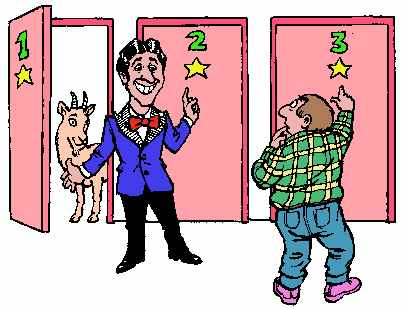
\includegraphics[width=5cm]{montyhall.jpg}}
%\\ \footnotesize Image from \url{http://www.grand-illusions.com/articles/monty_hall/}}

We use a causal Bayesian network to model this problem.
\begin{enumerate}
 \item Define a causal Bayesian network that fits with the story. Use the following variables:\\[0.5\baselineskip]
   \centerline{
   \begin{tabular}{ll}
     $C$:& initial choice (``choice'')\\
     $L$:& door behind which the prize is hidden (``location'')\\
     $D$:& door opened after you made your initial choice (``door'')\\
     $F$:& final choice after choosing to switch (or not)\\
     $I$:& node representing our strategy, $0$ if we do not switch, $1$ if we switch\\
     $O$:& what is behind the opened door of the final choice (``observation'')\\
   \end{tabular}}
   Clearly indicate the domain of each variable, which variables are observed, unobserved (at the moment just before you make your final choice) and input nodes. Explain your modeling choices. (1pt)
\item Define the discrete Markov kernel for each node of the Causal Graph corresponding to this problem. (1pt)
\item Calculate the probability of winning given do$(I=1)$ and do$(I=0)$. \emph{Hint:} You may use the fact that the problem is symmetric, and fix the initially chosen door to $1$. (1pt)
\end{enumerate}
Now let us change the story slightly. Suppose that before Monty can actually open a door (to show you that there is
a goat behind that door), an earthquake intervenes and happens to open one of the two doors that you didn't choose initially, and
you observe that there is a goat behind that door. Undisturbed by the earthquake, Monty thinks ``the show must go on!'' and proceeds
by asking you what your final choice is.
\begin{enumerate}[resume*]
  \item The earthquake intervention changes the causal Bayesian network. Draw the intervened causal Bayesian network (where we consider the earthquake as independently at random making a hard intervention on $D$). What is our win probability if we take Monty up on his offer in this case? (1pt)
  \item Write three simulation programs (where we highly recommend to practice in R), one where we \emph{stick}, one where we \emph{switch} after Monty opens a door, and one where we \emph{switch} after an earthquake opens a door (where we condition on the door opened not being a car, i.e. we throw away samples where the earthquake happened to open the door with the car). Explicitly model the generative process of the game. Use these simulations to estimate the win probability of each scenario using at least 1000 samples. (1pt)
\end{enumerate}

\begin{gradedsolution}
  \begin{figure}[ht]
    \centering
  \begin{tikzpicture}[scale=1, transform shape]
    \tikzstyle{every node} = [draw,shape=circle,color=blue]
    \node (L) at (4,0) {$L$};
    \node (D) at (2,0) {$D$};
    \node (F) at (2,-2) {$F$};
    \node (O) at (4,-2) {$O$};
    \tikzstyle{every node} = [draw,shape=rectangle,color=teal]
    \node (C) at (0,0) {$C$};
   \node (I) at (0,-2) {$I$};
   \draw[-{Latex[length=3mm, width=2mm]}, color=blue] (C) to (D);
   \draw[-{Latex[length=3mm, width=2mm]}, color=blue] (L) to (D);
   \draw[-{Latex[length=3mm, width=2mm]}, color=blue] (C) to (F);
   \draw[-{Latex[length=3mm, width=2mm]}, color=blue] (D) to (F);
   \draw[-{Latex[length=3mm, width=2mm]}, color=blue] (I) to (F);
   \draw[-{Latex[length=3mm, width=2mm]}, color=blue] (F) to (O);
   \draw[-{Latex[length=3mm, width=2mm]}, color=blue] (L) to (O);
  \end{tikzpicture}
  \caption{Causal graph $G$ corresponding to the Monty hall problem of exercise 4.}
  \label{fig:mh}
  \end{figure}
  \begin{enumerate}
    \item We have represented a possible graph for this problem in figure 3. The domains of all variables are given by $\{1,2,3\}$, except for $I$ and $O$ which have domain $\{0,1\}$ (where a $1$ for $O$ represents winning a car). Only $L$ is an unobserved variable. Note that representing both situations in a single graph loses some information compared to modeling two separate graphs: for example there is no arrow from $D$ to $F$ if $I=0$. In this graph we clearly see that knowledge about $L$ might influence our final choice through $D$.
    \item Firstly, $L$ has a discrete uniform distributions on its domain. We define the Markov kernel $P(D|Do(C, L)$ by two cases 
    \begin{itemize}
      \item If $c=l$ then it is the uniform distribution on $\{1,2,3\} \setminus \{c\}$. 
      \item If $c \neq l$, then $P(D=d|Do(C=c, L=l) = 1 - \delta_{\{c,l\}}(d)$.
    \end{itemize} 
    Similarly for the Markov kernel $P(F|Do(I, C, D)$ we distinguish cases:
    \begin{itemize}
      \item If $I=0$, then $P(F=f|Do(I=0, C=c, D=d) = \delta_{\{c\}}(f)$.
      \item If $I=1$, then by the generative process we only have to concern ourselves with the case where $c \neq d$, in which case $P(F=f|Do(I=0, C=c, D=d) = 1 - \delta_{\{c,d\}}(f)$. If $c = d$ we may define the Markov kernel as some arbitrary distribution over $F$.
    \end{itemize}  
     Finally, $P(O \given do(F, L))$ is defined by the probability mass function $P(O=1 \given do(F=f, L=l)) = \delta_{\{l\}}(f)$.
     \item First consider the case if $I=0$. Then $F=C$ and the probability reduces to whether $L=C$ which is $1/3$ since its discretely uniformly distributed.\\
     
     Now consider the case where $I=1$. With probability $1/3$ it will be the case that $L=1$, in which case both $D$ and $F$ will be $2$ or $3$, and we will lose the game. However, with probability $2/3$ we will have that $L=\neq 1$, in which case $F=L$ and we will win the game. Thus the probability of winning is thus $2/3$ when we switch.
     \item The graph after earthquake intervention is shown in figure 4. It is clear since $F$ has to match $L$ and $L$ is independently drawn, that the win probability is the same for all strategies, i.e. the probability of winning is $1/2$ since there are now $2$ doors to choose from. Conditioning on $D$ does not open a path.
  \end{enumerate}
  
  \begin{figure}[ht]
    \centering
  \begin{tikzpicture}[scale=1, transform shape]
    \tikzstyle{every node} = [draw,shape=circle,color=blue]
    \node (L) at (4,0) {$L$};
    \node (F) at (2,-2) {$F$};
    \node (O) at (4,-2) {$O$};
    \tikzstyle{every node} = [draw,shape=rectangle,color=teal]
    \node (C) at (0,0) {$C$};
    \node (D) at (2,0) {$D$};
   \node (I) at (0,-2) {$I$};
   \draw[-{Latex[length=3mm, width=2mm]}, color=blue] (C) to (F);
   \draw[-{Latex[length=3mm, width=2mm]}, color=blue] (D) to (F);
   \draw[-{Latex[length=3mm, width=2mm]}, color=blue] (I) to (F);
   \draw[-{Latex[length=3mm, width=2mm]}, color=blue] (F) to (O);
   \draw[-{Latex[length=3mm, width=2mm]}, color=blue] (L) to (O);
  \end{tikzpicture}
  \caption{Causal graph $G$ corresponding to the Monty hall problem of exercise 4 after the earthquake intervention.}
  \label{fig:mh2}
  \end{figure}
\end{gradedsolution}

\section*{R code for Monty Hall problem normal variant}
\begin{lstlisting}[language=R]
initial_choice <- sample(c(1,2,3),1000, replace=TRUE)
car <- sample(c(1,2,3),1000, replace=TRUE)

# Define a function that given a combination of initial_choice 
# and car samples door correctly
f1 <- function(ic,ca) {
    space <- c(1,2,3)
    if (ic == ca) {
        return(sample(space[space != ic],1, replace=TRUE))
    } else {
        return(space[space != ic & space != ca])
    }
}
# Apply this to the combination of initial_choice and car vectors
door <- mapply(f1, initial_choice,car)

# Switch or do not switch:
final_choice_stick <- initial_choice
final_choice_switch <- 1*(initial_choice != 1 & door != 1) + 
                        2*(initial_choice != 2 & door != 2) + 
                        3*(initial_choice != 3 & door != 3)

# Calculate win probabilities
print(mean((final_choice_switch == car)))
print(mean((final_choice_stick == car)))
  \end{lstlisting}
  \section*{R code for Monty Hall problem earthquake intervention}
  \begin{lstlisting}[language=R]
initial_choice <- sample(c(1,2,3),5000, replace=TRUE)
car <- sample(c(1,2,3),5000, replace=TRUE)
door <- sample(c(1,2,3),5000, replace=TRUE)

mask <- (door != initial_choice) & (door != car) 

final_choice_switch <- 1*(initial_choice != 1 & door != 1) + 
                    2*(initial_choice != 2 & door != 2) + 
                    3*(initial_choice != 3 & door != 3)

final_choice_stick <- initial_choice

print(mean((final_choice_switch == car)[mask]))
print(mean((final_choice_stick == car)[mask]))
\end{lstlisting}
\end{document}
